%************************************************
%\chapter{Distinction of drivers in pCO$_2$} % $\mathbb{ZNR}$
\chapter{Contribution of different processes to multi-year pCO$_2$ trends} % $\mathbb{ZNR}$
%
%************************************************
\label{ch:pCO2separation}

%\paragraph{Purpose of pCO$_2$ separation}
%\subsection{Explanation and assuof the framework and its assumptions}
The previous analysis of thermal, circulation and biological CO$_2$ flux responses towards the westerly winds in \autoref{ch:trends} asks for an estimate on the relative contributions of each process to the total change. As all the processes interact with each other non-linearly, a clear and clean separation cannot be taken in precision. Therefore the results of this chapter must be understood rather as an \textit{estimation of the first-order drivers} in pCO$_2$. In this chapter I adapt the pCO$_2$ diagnostics framework from \citeauthor{Lovenduski2007} [{\color{RoyalBlue}2007}] to quantitatively estimate the different contributions to pCO$_{\text{2,ocean}}$ and thus sea-air CO$_2$ flux changes.

\section{Derivation of the framework}
%The framework assumes a well-mixed euphotic zone zonal carbon budget box, where \acs{DIC} enters at the upper boundary via sea-air CO$_2$ flux, freshwater input changes \acs{DIC} and alkalinity concentrations, \acs{DIC} and alkalinity leave the system at the lower boundary via biology export production (fig. \ref{fig:pCO2_separation}). Furthermore, changes in pCO$_2$ due to changes in salinity and \acs{SST} are accounted for and the residual is interpreted. Based on the individual processes taking place, a change in pCO$_2$ due to that process is calculated from monthly model output data.\newline

%neu
The framework relies on a well-mixed alkalinity and carbon budget across zonal bands of 10$^\circ$ latitude from 50-60$^\circ$S and 40-50$^\circ$S of the upper ocean upto the \acf{MLD} (\autoref{fig:pCO2_separation}). pCO$_{\text{2,ocean}}$ changes associated with different processes are calculated from month-ly model output data.\newline

\begin{figure}[hbt]
	\centering
	\includegraphics[scale=.51,page=2,trim=5.cm 5.7cm 2.7cm 2.3cm,clip]{co2sep}
	\caption{Schematic illustration of pCO$_2$ driver separation assuming a well-mixed zonal box, where changes in pCO$_{\text{2,ocean}}$ are separated into contributions due to sea-air CO$_2$ flux (red), thermal effect (orange), the saline effect (yellow), freshwater (light blue), biology (green) and a residual (dark blue)}	
	\label{fig:pCO2_separation}
\end{figure}

I separate pCO$_{\text{2,ocean}}$ into different perspectives of understanding: The first perspective on the changes in dissociation constants and solubility separates contributions in the thermal and the saline effect. The second perspective associates pCO$_{\text{2,ocean}}$-changes with concentration changes in alkalinity (Alk) and \acs{DIC}. 

\begin{align}
\allowdisplaybreaks
\delta pCO_{\text{2,ocean}}&=\underbrace{\delta pCO_{\text{2,thermal}}+\delta pCO_{\text{2,sal}}}_{\text{dissociation constants and solubility changes}} \notag \\
&\phantom{{}={}} +\underbrace{\delta pCO_{\text{2,non-thermal-sal}}}_{\text{concentration changes}}  \\
\delta pCO_{\text{2,non-thermal-sal}}&\approx \delta pCO_{\text{2,Alk}}+\delta pCO_{\text{2,DIC}}
\end{align}

The thermal separation from \citeauthor{Takahashi1993} [{\color{RoyalBlue}1993};  {\color{RoyalBlue}2002}] identifies a thermal pCO$_{\text{2,thermal}}$ from pCO$_{\text{2,ocean}}$ (\autoref{eq:thermal}). This empirical fit describes the changes in pCO$_{\text{2,ocean}}$ of a warming water parcel, \ie how the temperature-dependent equilibrium constants and solubility change the pCO$_{\text{2,ocean}}$ at constant salinity, \acs{DIC} and alkalinity. 

The salinity dependence for constant \acs{DIC}, alkalinity and \acs{SST} describes the changes of dissociation constants due to changes in salinity (\autoref{eq:saline}), so an increase in salinity increases pCO$_{\text{2,ocean}}$ \citep{Sarmiento2006}. The non-thermal-saline residual (\autoref{eq:non-thermal-saline}) covers the changes of all other processes, which vary pCO$_{\text{2,ocean}}$ excluding the thermal and saline effect, namely concentration changes in \acs{DIC} and alkalinity:
\begin{align}
\allowdisplaybreaks
\delta pCO_{\text{2,thermal}}&\approx \frac{\partial pCO_2}{\partial T}\cdot \delta T \approx \overline{pCO_2} \cdot 0.0423 ^{\circ}C^{-1} \cdot \delta T \label{eq:thermal}\\
\delta pCO_{\text{2,sal}}&=\frac{\partial pCO_2}{\partial S}\cdot \delta S \approx \frac{\overline{pCO_2}}{\overline{S}} \cdot \underbrace{\gamma_{S}}_{\approx 1} \cdot \delta S \label{eq:saline}\\
\delta pCO_{\text{2,non-thermal-sal}} &= \delta pCO_{\text{2,ocean}}-\delta pCO_{\text{2,therm}}-\delta pCO_{\text{2,sal}} \label{eq:non-thermal-saline}
\end{align}

For a deeper look into the pCO$_{\text{2,ocean}}$ due to non-thermal-saline effects (\autoref{eq:non-thermal-saline}), I use the salinity-normalized concentrations sDIC and sAlk for \acs{DIC} and alkalinity to prevent double-accounting of freshwater (FW) changes in \acs{DIC} and alkalinity \citep{Keeling2004}:
\begin{align}
\allowdisplaybreaks
sDIC&=\frac{DIC}{S}\cdot S_0  \text{ }\text{ }\text{ }\text{ }\text{ }\text{ }\text{ }\text{ }\text{ }\text{ } S_0=35 \text{ psu} \\
\delta pCO_{\text{2,non-thermal-sal}} &\approx \frac{\partial pCO_2}{\partial (S/S_0 \text{ } sAlk)}\delta (S/S_0 \text{ } sAlk) \notag \\
&\phantom{{}={}} + \frac{\partial pCO_2}{\partial (S/S_0 \text{ } sDIC)}\delta (S/S_0 \text{ } sDIC) \\
&\approx \frac{S}{S_0}\frac{\partial pCO_2}{\partial Alk}\delta sAlk + \frac{S}{S_0}\frac{\partial pCO_2}{\partial DIC}\delta sDIC \notag \\
&\phantom{{}={}}+ \frac{\partial pCO_2}{\partial FW}\delta FW \label{eq:where_fw}
\end{align}

%\begin{align*}
%\delta pCO_2&=\delta pCO_{\text{2,thermal}}+\delta pCO_{\text{2,salt}}+\delta pCO_{\text{2,alk}}+\delta pCO_{\text{2,DIC}} \\ \\
%&= \frac{\partial pCO_2}{\partial T}\delta T + \frac{\partial pCO_2}{\partial S}\delta S  + \frac{S}{S_0}\frac{\partial pCO_2}{\partial Alk}\delta sAlk  \\ &+ \frac{S}{S_0}\frac{\partial pCO_2}{\partial DIC}\delta sDIC + \frac{\partial pCO_2}{\partial FW}\delta FW. 
%\end{align*}
pCO$_{\text{2,ocean}}$ increases for increasing \acs{DIC} and decreases for increasing alkalinity: %The sensitivities of pCO$_{\text{2,ocean}}$ towards changes in \acs{DIC} and alkalinity are taken from \cite{Sarmiento2006}: 
%\allowdisplaybreaks
\begin{align}
\frac{\partial pCO_2}{\partial DIC} &= \frac{pCO_2}{DIC} \cdot \gamma_{DIC} \\
\frac{\partial pCO_2}{\partial Alk} &= \frac{pCO_2}{Alk} \cdot \gamma_{Alk} 
\end{align}
It is noteworthy that sensitivity factors $\gamma_{DIC}$ and $\gamma_{Alk}$ are approximations, because they are partial derivatives from a simplified pCO$_{\text{2,ocean}}$ formulation by substituting bicarbonate and carbonate ion concentrations with \acs{DIC} and alkalinity \citep[p. 328]{Sarmiento2006}:  
\begin{align}
\allowdisplaybreaks
\gamma_{DIC} &\approx \frac{3 \cdot Alk \cdot DIC - 2 \cdot DIC^2}{(2 \cdot DIC - Alk)(Alk-DIC)} \label{eq:gamma_dic}\\
\gamma_{Alk} &\approx -\frac{Alk^2}{(2 \cdot DIC - Alk)(Alk-DIC)} \label{eq:gamma_alk}
\end{align}
 
Additional freshwater input (\autoref{eq:where_fw}) reduces the concentration of \acs{DIC}, alkalinity and salinity by dilution and leads to a slight decrease in pCO$_{\text{2,ocean}}$. Vice versa, net evaporation increases the concentration of \acs{DIC}, alkalinity and salinity and thus increases pCO$_{\text{2,ocean}}$:
\begin{align}
\allowdisplaybreaks
\frac{\partial pCO_2}{\partial FW} &= \frac{sDIC}{S_0}\frac{\partial pCO_2}{\partial DIC}\delta S + \frac{sAlk}{S_0}\frac{\partial pCO_2}{\partial Alk}\delta S
\end{align}

%\begin{align*}
%\allowdisplaybreaks
%\frac{\partial pCO_2}{\partial FW} &= \frac{pCO_2}{MLD} \cdot \gamma_{FW} \\
%\gamma_{FW}&=\gamma_{Alk}+\gamma_{DIC}+\gamma_{S}
%\end{align*}

Furthermore the changes in sDIC and sAlk are separated into biological, sea-air exchange and residual contribution to check for the origin of \acs{DIC} and alkalinity changes, \ie biological export, sea-air CO$_2$ flux or other not specified processes as the residual (likewise for $\delta sAlk$):

\begin{align}
\frac{\delta (\text{sDIC})}{\delta t}=\frac{\delta (DIC_{\text{bio}})}{\delta t}+\frac{\delta (DIC_{\text{exchange}})}{\delta t}+\frac{\delta (sDIC_{\text{res}})}{\delta t}
\end{align}

The changes due to sea-air CO$_2$ flux and biology are converted to \acs{DIC} and alkalinity concentration changes by dividing by the \ac{MLD} assuming that the concentration changes are well-mixed across the mixed layer. This assumes that the system is in a steady state and only changes in CO$_2$ flux, biological export and the residual affect the pCO$_{\text{2,ocean}}$ trend.

Furthermore, the concentration change of biological primary production and remineralization contributes with organic matter export (coex) and calcium carbonate export (caex) to changes in \acs{DIC} and alkalinity. 
Organic matter production reduces \acs{DIC} and increases alkalinity. Calcification increases \acs{DIC} and reduces alkalinity by two units by consuming the carbonate ion (Ca$^{++}$). The magnitude of conversion factors arise from the fixed Redfield stoichmetry ($C:N:P = 122:$ $16:1$) converting carbon to phosphate units in which alkalinity is accounted for. %Inventory changes in \acf{DOC} contribute as the organic matter pump [reason?!]. 
For a representation of the pCO$_{\text{2,ocean}}$ responses of the different processes see \autoref{fig:deffeyes_processes}.

\begin{align}
\delta DIC_{bio}&=-\frac{coex+caex}{MLD} \label{eq:mld}\\
\delta Alk_{bio}&=-\frac{2 \cdot caex-16/122 \cdot coex}{MLD}
\end{align}

The resulting sea-air CO$_2$ flux reflects the pCO$_{\text{2,ocean}}$ after being exposed to all changes by biology and circulation. By definition, CO$_2$ is also temperature-dependent in $k_w$ and reduces the \acs{DIC} concentration without changing alkalinity (\autoref{sec:HAMOCC}):
\begin{align}
\delta DIC_{ex}&=-\frac{CO_2 flux}{MLD} \label{eq:mlde} \\
\delta Alk_{ex}&=0
\end{align}
%\vspace{1cm}

These concentration changes in \acs{DIC} and alkalinity modify pCO$_{\text{2,ocean}}$ at the same time.  The \acs{DIC} and alkalinity contribute with different $\gamma$ sensitivities and add up to the combined pCO$_{\text{2,ocean}}$ change,\eg the total pCO$_{\text{2,bio}}$ change combines pCO$_{\text{2bio,DIC}}$ and pCO$_{\text{2,bio,Alk}}$.\newline

The remaining salinity-corrected residual pCO$_{\text{2,res}}$ accounts for all other processes not covered in this framework and approximative errors: 
\begin{itemize}
%\item[-] negligible errors in approximations used during derivation
\item[-] vertical and lateral advection of \acs{DIC} and alkalinity
\item[-] changes in biological carbon inventory
\item[-] lateral advection of organic tracers
\item[-] linearizations of non-linear processes
\item[-] calculation from monthly timesteps
\item[-] simplification of $\gamma$ sensitivity constants in \cite{Sarmiento2006} (\autoref{eq:gamma_dic}, \ref{eq:gamma_alk})
\item[-] non-steady state in the beginning of the period
%\item[-] residual as combined contribution of everything which is not described, mainly vertical and lateral circulation, but also to a lesser degree advection of biological constituents
%\item[-] ignoring time-averaging inconsistency: monthly mean offline instead of instantaneous online calculation
%\item[-] well-mixed mixed layer
\end{itemize}



\clearpage
\section{Estimate of pCO$_2$ drivers}


Applying the above described framework yields an estimation for the drivers of pCO$_2$ for the two extreme trends into the two latitudinal regions each with opposing responses from \autoref{ch:trends}  (\autoref{tab:trends_pco2}). In this section I analyze the positive and negative pCO$_{\text{2,ocean}}$ trends first under the perspective of dissociation constants and solubility changes, and then to gain further insights on the non-thermal-saline part under the perspective of concentration changes. Concluding, I frame a picture of the $\Delta$pCO$_2$ changes and thus sea-air CO$_2$ flux.

\begin{table}[hbt]
\centering
\begin{tabular}{ l | c c | c c}
\multicolumn{5}{l} {8-yr trend} {\hspace{1.cm} 50-60$^\circ$S \hspace{2.cm} 40-50$^\circ$S} \hspace{1.cm} \\ \hline
%{8-yr trend} \multicolumn{2}{l} 50-60$^\circ$S \multicolumn{2}{l} 40-50$^\circ$S} \\ \hline
  pCO$_{\text{2,x}}$  [ppm] & positive  & negative & positive  & negative  \\
  \hline  
  pCO$_{\text{2,thermal}}$ & -7.1 & 6.7 & 3.4 & 0.7 \\    
  pCO$_{\text{2,sal}}$ & 0.6 & -0.5 & 0.2 & -0.3 \\  
  pCO$_{\text{2,non-thermal-sal}}$ & 38.4 & -8.7 & 6.4 & 12.5  \\
  \hline \hline
  pCO$_{\text{2,FW}}$ & 0.6 & -0.5 & 0.2 & -0.3 \\
  pCO$_{\text{2,sDIC}}$ & 37.6 & 1.0 & 10.6 & 19.1 \\
  pCO$_{\text{2,sAlk}}$ & 8.1 & -4.2 & -1.8 & -1.5 \\
  \hline 
  pCO$_{\text{2,ex,DIC}}$ & -5.1 & 5.2 & 0.2 & 1.1 \\
  \hline
  %%%new bio summer
  pCO$_{\text{2,bio,DIC}}$ & 4.9 & -6.2 & -1.4 & -0.1 \\
  pCO$_{\text{2,bio,Alk}}$ & 0.5 & -0.6 & -0.1 & -0.0 \\
  \hline
  pCO$_{\text{2,bio}}$ & 5.4 & -6.8 & -1.5 & -0.1 \\
%%%% 
%  pCO$_{\text{2,bio,DIC}}$ & 2.7 & -3.4 & -0.8 & -0.2 \\
%  pCO$_{\text{2,bio,Alk}}$ & 0.3 & -0.3 & -0.1 & -0.0 \\
%  \hline
%  pCO$_{\text{2,bio}}$ & 3.0 & -3.7 & -0.9 & -0.2 \\
 
  \hline
  pCO$_{\text{2,res,sDIC}}$ & 40.0 & -0.8 & 9.8 & 18.2  \\
  pCO$_{\text{2,res,sAlk}}$ & 7.8 & -3.9 & -1.7 & -1.5 \\
  \hline
  pCO$_{\text{2,res}}$ & 47.8 & -4.7 & 8.1 & 16.7 \\
  \hline \hline
  pCO$_{\text{2,ocean}}$ & 32.1 & -2.4 & 9.4 &  12.9 \\
  pCO$_{\text{2,atm}}$ & 12.0 & 14.5 & 12.0 &  14.5 \\
  \hline \hline
  dpCO$_{\text{2}}$ & 20.2 & -16.9 & -2.6 & -1.6  \\
\end{tabular}
\caption{Trends in drivers of pCO$_2$ for the most positive sea-air CO$_2$ flux trend and the most negative sea-air CO$_2$ flux trend in two 10$^\circ$-\ac{MLD} boxes. Only austral summer months contribute to biological trends (pCO$_{\text{2,bio}}$).}
\label{tab:trends_pco2}
\end{table}

%positive trend
%50-60$^\circ$S
%thermal non-thermal
%ein ausfuerhlicher durchlauf, danach fixer
During the most positive sea-air CO$_2$ flux trend at 50-60$^\circ$S, the thermal trend (pCO$_{\text{2,thermal}}$) decreased because of sea-surface cooling and drives carbon uptake (\autoref{sec:trends_pos_thermal}). While salinity changes (pCO$_{\text{2,sal}}$) are negligible, the overall trend (pCO$_{\text{2,ocean}}$) opposes the thermal trend (pCO$_{\text{2,thermal}}$). So changes in dissociation constants in the thermal and saline effect do not drive this pCO$_{\text{2,ocean}}$ trend but changes in concentration (pCO$_{\text{2,non-thermal-sal}}$).

%DIC,alk
The perspective on processes changing \acs{DIC} and alkalinity reveals that concentration (the opposite process to dilution, see \autoref{fig:deffeyes_processes}) of \acs{DIC} and alkalinity (pCO$_{\text{2,FW}}$) has only a minor effect. The largest contribution to the pCO$_{\text{2,ocean}}$ trend arises from the changes in salinity-normalized alkalinity (pCO$_{\text{2,sAlk}}$) and mostly \acs{DIC} (pCO$_{\text{2,sDIC}}$). As outgassing increases, \acs{DIC} (pCO$_{\text{2,ex,DIC}}$) increasingly leaves the system and thereby decreases pCO$_{\text{2,ocean}}$. For biological processes I take only the summer trends as phytoplankton does not bloom in winter. It comprises mostly organic matter production which decreases and therefore exports less carbon and more alkalinity out of the system all-in-all increasing pCO$_{\text{2,ocean}}$ (\autoref{sec:trends_pos_biology}). The remaining residual in \acs{DIC}-driven (pCO$_{\text{2,res,sDIC}}$) and alkalinity-driven (pCO$_{\text{2,res,sAlk}}$) trends, which are not covered by a distinct process in this framework, dominate this concentration-driven (pCO$_{\text{2,non-thermal-sal}}$) trend. Therefore at this instance, biology (pCO$_{\text{2,bio}}$) plays only a minor role and is likely outplayed by circulation changes (pCO$_{\text{2,res}}$). The changes due to upwelling are very dependent on the history of the water masses advected into and out of the system. Generally, deeper waters have higher \acs{DIC} and alkalinity concentrations in the Southern Ocean and \acs{DIC} would have a slightly higher impact on pCO$_{\text{2,ocean}}$ because of slightly higher $\gamma_{\text{DIC}}$, but the proportions of \acs{DIC} and alkalinity matter. So here a strong increase in \acs{DIC} increases pCO$_{\text{2,res,sDIC}}$ while the increase in alkalinity reduces pCO$_{\text{2,res,sAlk}}$. These changes are either due to advection changes or an underestimation of the organic matter production decrease (pCO$_{\text{2,bio}}$). The trends in advection of both \acs{DIC} (pCO$_{\text{2,res,sDIC}}$) and alkalinity (pCO$_{\text{2,res,sAlk}}$) are negative, so while upwelling could explain the the \acs{DIC} (pCO$_{\text{2,res,sDIC}}$) trend, a clear attribution of upwelling to alkalinity (pCO$_{\text{2,res,sAlk}}$) cannot be made here (\autoref{sec:trends_pos_circulation}).\newline

%40-50$^\circ$S
%thermal non-thermal
At 40-50$^\circ$S, the warming trend increases $pCO_{\text{2,thermal}}$, which drives CO$_2$ outgassing (\autoref{sec:trends_pos_thermal}). Also the contributions unrelated to dissociation constants changes (pCO$_{\text{2,non-thermal-sal}}$) increase but at a higher rate. 

%DIC,alk
Looking deeper into these contributions biology slightly increases, so pCO$_{\text{2,bio}}$ decreases (\autoref{sec:trends_pos_biology}), while changes in air-sea CO$_2$ flux (pCO$_{\text{2,ex,DIC}}$) are negligible. Overall the residual (pCO$_{\text{2,res,sAlk}}$) dominates again. Here, unaccounted processes  increase \acs{DIC} and alkalinity, so pCO$_{\text{2,res,sDIC}}$ increases and pCO$_{\text{2,res,sAlk}}$ decreases. pCO$_{\text{2,res,sDIC}}$ drives the pCO$_{\text{2,ocean}}$ trend. As advection increases \acs{DIC} and alkalinity this is related to the circulation changes (\autoref{sec:trends_pos_circulation}).\newline

%combined pic
\label{sec:pCO2separation_pos}
Combining the pCO$_{\text{2,ocean}}$ responses for the most extreme positive CO$_2$ flux trend with the atmospheric pCO$_{\text{2,atm}}$ changes lead me to a comprehensive CO$_2$ flux picture (\autoref{fig:schematics_pos}). 

While the cooling effect of the stronger winds reduces outgassing in the high-latitude Southern Ocean, the decline in primary production and mostly the increasing upwelling of deeper waters and outplay the thermal effect to a strong positive pCO$_{\text{2,ocean}}$ trend at 50-60$^\circ$S. 
At 40-50$^\circ$S the warming effect reduces carbon uptake, which outweighs the non-thermal-saline changes, namely increasing \acs{DIC} due to lateral advection and less downwelling (with negligible contributions from sea-air CO$_2$ flux and biology), which leads to a combined positive pCO$_{\text{2,ocean}}$ trend. 

The atmospheric trend pCO$_{\text{2,atm}}$ is strictly positive and sets $\Delta$pCO$_{2}$ to a still strong positive trend at 50-60$^\circ$S and a weak decreasing trend at 40-50$^\circ$S. 
The resulting outgassing CO$_2$ flux trend at 50-60$^\circ$S is stronger than the weak CO$_2$ uptake trend at 40-50$^\circ$S and hence determines the overall Southern Ocean carbon sink trend. The overall positive CO$_2$ flux trend and its opposite thermal contributions agree with \cite{Lovenduski2007}.\newline

\begin{figure}[hbt]
	\centering
	\includegraphics[scale=.65,trim=3.5cm 2.5cm 7.5cm 0.5cm,clip,page=17]{SO_schematics}
	\caption{Schematic illustration of the Southern Ocean under the context of increasing westerly winds and response in the thermal effect, biology and upper-ocean circulation lead towards a positive sea-air CO$_2$ flux trend; red color-coding indicates a relative increase of the related quantity or process, whereas blue indicates a relative decrease. The grey line represents the \acf{MLD} in the beginning of the trend period, the black line the \acs{MLD} in the end of the trend period.}
	%\caption{Schematic illustration of the Southern Ocean under the context of increasing westerly winds and response in the thermal effect, biology and upper-ocean circulation leading towards a positive CO$_2$ flux trend; red color-coding indicates a relative increase of the related quantity or process, whereas blue indicates a relative decrease. Stronger winds enhance the upper-ocean overturning circulation. Increased upwelling increases outgassing of over-saturated deep waters. Increased Ekman transport advects \acs{DIC} further north, cools the higher latitudes and warms the lower latitudes. Deeper mixing and cooling in the higher latitudes decreases primary production, whereas shallower mixing and warming increase primary production in the lower latitudes. Combined with increasing atmospheric pCO$_2$, the higher latitude outgas strongly, whereas the lower-latitudes slightly ingas.}
	\label{fig:schematics_pos}
\end{figure}

\clearpage

%negative trend
%50-60$^\circ$S
%thermal non-thermal
During the most negative sea-air CO$_2$ flux trend at 50-60$^\circ$S, the thermal trend (pCO$_{\text{2,thermal}}$) decreased due to sea-surface warming (\autoref{sec:trends_neg_thermal}), the saline effect (pCO$_{\text{2,sal}}$) is negligible, but the thermal and saline effects are overcompensated by concentration changing processes (pCO$_{\text{2,non-thermal-sal}}$). But this is of far less extent than for the most positive sea-air CO$_2$ flux trend, as the overall pCO$_{\text{2,ocean}}$ only slightly decreases.
%DIC,alk
The contribution of \acs{DIC} (pCO$_{\text{2,sDIC}}$) increases only slightly, whereas the contribution from alkalinity (pCO$_{\text{2,sAlk}}$) dominates the negative trend. Looking into the individual processes, increased CO$_2$ uptake (pCO$_{\text{2,ex,DIC}}$) increases, whereas increased biology (pCO$_{\text{2,bio}}$) reduces pCO$_{\text{2,ocean}}$. The residual \acs{DIC} contribution (pCO$_{\text{2,res,DIC}}$) slightly decreases as does \acs{DIC} advection (\autoref{sec:trends_pos_circulation}) which could attribute the residual \acs{DIC} to decreased upwelling. The residual alkalinity contribution (pCO$_{\text{2,res,sAlk}}$) decreases stronger, but the concentration changes in alkalinity due to advection also decline, so a clean attribution of residual alkalinity changes to advective circulation changes cannot be made here.  

%40-50$^\circ$S
%thermal non-thermal
At 40-50$^\circ$S the thermal trend (pCO$_{\text{2,thermal}}$) remains almost unaltered and slightly increases (\autoref{sec:trends_neg_thermal}). The major trend in pCO$_{\text{2,ocean}}$ outgassing arises from concentration changes (pCO$_{\text{2,non-thermal-saline}}$). 

%DIC,alk
Changes in \acs{DIC} (pCO$_{\text{2,sDIC}}$) strongly lead this outgassing trend by a strong residual \acs{DIC} (pCO$_{\text{2,res,DIC}}$) increase, which comes from increased \acs{DIC} concentrations due to advection, namely less northward advection and reduced downwelling. This reduced downwelling may be a sign of increased upwelling caused by the northward shift of the overturning cell over the 40$^\circ$S boundary. The same applies for increased alkalinity, where (pCO$_{\text{2,res,sAlk}}$) reduces pCO$_{\text{2,ocean}}$ slightly. These residual changes (pCO$_{\text{2,res}}$) are clear signs of upwelling.\newline


%\paragraph{negative CO$_2$ flux trend}
\label{sec:pCO2separation_neg}
The three distinct pCO$_2$ responses for the most negative CO$_2$ flux trend merge with the rising atmospheric pCO$_{\text{2,atm}}$ into the opposing picture in CO$_2$ flux as for decreasing westerly winds (\autoref{fig:schematics_neg}). 

Weaker winds warm the high-latitude Southern Ocean, which leads to outgassing, but the decreasing upwelling and the decline in primary production outplay the thermal effect to a relative ingassing trend at 50-60$^\circ$S. At 40-50$^\circ$S temperatures remain constant and decreased Ekman transport \acs{DIC} supply and increased northward-shifted upwelling leads to a combined relative pCO$_{\text{2,ocean}}$ outgassing trend. 

The strictly positive atmospheric trend $pCO_{\text{2,atm}}$ outperforms the slightly negative pCO$_{\text{2,ocean}}$ trend at 50-60$^\circ$S and slightly overcompensates the pCO$_{\text{2,ocean}}$ positive trend at 40-50$^\circ$S. The resulting negative sea-air CO$_2$ flux signal at 50-60$^\circ$S is stronger than the slightly positive sea-air CO$_2$ flux at 40-50$^\circ$S and hence determines the overall Southern Ocean carbon sink trend.\newline

% trend.  is strictly positive and sets $\Delta pCO_{2}$ to a still strong positive trend at 50-60$^\circ$S and a weak decreasing trend at 40-50$^\circ$S. The resulting outgassing CO$_2$ flux trend at 50-60$^\circ$S is stronger than the weak CO$_2$ uptake trend at 40-50$^\circ$S and hence determines the overall Southern Ocean carbon sink trend. The overall positive CO$_2$ flux trend and its opposite thermal contribution agrees with \cite{Lovenduski2007}.\newline

\begin{figure}[hbt]
	\centering
	\includegraphics[scale=.65,trim=3.5cm 2.5cm 7.5cm 0.5cm,clip,page=18]{SO_schematics}
	\caption{Schematic illustration of the Southern Ocean under the context of decreasing westerly winds and response in the thermal effect, biology and upper-ocean circulation leading towards a negative sea-air CO$_2$ flux trend; red color-coding indicates a relative increase of the related quantity or process, grey indicates no changes and blue indicates a relative decrease. The grey line represents the \acf{MLD} in the beginning of the trend period, the black line the \acs{MLD} in the end of the trend period.}
	%\caption{Schematic illustration of the Southern Ocean under the context of decreasing westerly winds and response in the thermal effect, biology and upper-ocean circulation leading towards a negative CO$_2$ flux trend; red color-coding indicates a relative increase of the related quantity or process, whereas blue indicates a relative decrease. Weaker and northward-shifted winds decrease the upper-ocean overturning circulation, increase primary production at higher latitudes because of deeper mixing and warming. Decreased Ekman transport warms the higher latitudes and reduces Ekamn advection, but northward-shifted upwelling increases. Combined with rising atmospheric pCO$_2$, the higher latitudes strongly ingas, whereas the lower-latitudes slight ingas.}
	\label{fig:schematics_neg}
\end{figure}

\clearpage
%main findings

Summarizing, the framework shows the asymmetric contributions of the different drivers in the positive and negative trend (\autoref{tab:trends_pco2}). The contribution due to changes in salinity-normalized \acs{DIC} changes (pCO$_{\text{2,sDIC}}$) has a very strong influence and is not symmetric towards zero. pCO$_{\text{2,sDIC}}$ mostly reflects the changes in lateral and vertical transport of \acs{DIC}. Acknowledging that the system is not in steady-state but under transient historical forcing of increasing atmospheric in pCO$_{\text{2,atm}}$, pCO$_{\text{2,sDIC}}$ is expected to rise because the water masses flowing laterally into the budget box are affected by CO$_2$ uptake by the oceans. In the non-varying carbon uptake state, the expected pCO$_{\text{2,sDIC}}$ due to lateral transports could be estimated to the increasing pCO$_{\text{2,atm}}$ of $\sim12-14$ ppm/8yrs. Considering this, also pCO$_{\text{2,sDIC}}$ responds symmetric.\newline

%discussion of sensitivities of the framework
The framework is very susceptible in the magnitude of individual contributions for the definition of the depth of mixing in \autoref{eq:mld}-\ref{eq:mlde}, \ie whether I choose the top layer of $\sim12m$, fixed $90 m$, or the actually taken varying \acf{MLD}. The direction of the described processes and their relative contributions do not change and the residual adjusts accordingly.

The changes in inventory related to biology is estimated from the change of concentrations from  phytoplankton, zooplankton, acf{DOC} and detritus in carbon units, which make upto $\sim$10\%  additionally to the biological pCO$_{\text{2,ocean}}$ change, but cannot be quantified consistently as the fraction of calcifiers is unknown.

The attribution of the residual changes in \acs{DIC} to advective changes works at 40-50$^\circ$S but lacks the clear link at 50-60$^\circ$S. The trends in alkalinity transport are close to the trends in \acs{DIC} transport (as in \autoref{fig:UOOC_pos} and \autoref{fig:UOOC_neg}). Therefore, the pCO$_{\text{2,ocean}}$ trends in the same direction cannot be explained entirely by advective circulation changes. Also the steady state assumption, which is necessary for this box model approach, might shift the framework to misleading responses, because those strong trends cannot start from equilibrium in a transient simulation (\autoref{fig:evolution_southern_ocean_carbon_sink}). Nevertheless, the framework demonstrates that the strongest contribution of the pCO$_{\text{2,ocean}}$ trends arises from a process not explicitly specified in the framework, which is most probably the sum of changes in vertical and lateral advection.

%%%OLD
%In broad terms, the trends reverse for opposite wind forcing and the area 50-60$^\circ$S sets the trend of the overall Southern Ocean carbon sink south of 35$^\circ$S. The change in sDIC and sAlk dominate over the thermal, dilution and saline effect. The changes in pCO$_2$ due to biology and temperature are much smaller than the residual change. So, the major contributor to the pCO$_2$ is neither biology nor temperature, but not directly accounted for. Most likely changes in ocean circulation account for this residual and therefore highly depend on the history of the water masses which enter my box of interest. Here, the sDIC contribution dominates over the sAlk contribution (expect for negative trend at 50-60$^\circ$S).%note on seasonality

%Overall, biology seems more susceptible to wind-driven changes at 50-60$^\circ$S than 40-50$^\circ$S, this separation might be biased by the selection of the latitudinal boundaries.\newline

%In detail, the ongoing processes do not simply reverse as the atmospheric forcing trend stays the same. 
%The most positive CO$_2$ flux trend is mainly driven by the non-thermal pCO$_{\text{2,ocean}}$ ocean changes, whereas the most negative CO$_2$ flux trend is mainly driven by the increasing pCO$_{\text{2,atm}}$ concentrations, when the oceanic pCO$_{\text{2,ocean}}$ only has a very weak uptake trend and the upper-ocean overturning cell shifts northward.

%In the negative CO$_2$ flux trend, pCO$_{\text{2,ocean}}$ due to circulation increases at 40-50$^\circ$S, whereas less Ekman transport would predict a decrease. Here for the northward shift of the westerlies, the upwelling cell migrated northwards and thus increased the entrainment of carbon-rich waters. Also the warming extends further north into the area of 40-50$^\circ$S, which shifts the increasing pCO$_{\text{2,ocean}}$ trend from cooling out of 40-50$^\circ$S, resulting in a positive thermal trend.


